\chapter{Appendix A: Additional Details}
\label{appendix:a}
% Add content for Appendix A here
\section{Pairwise Correlations}
\label{sec:pairwise_corr_unambiguous}

\begin{table}[h!]
\centering
\begin{tabular}{|l|c|c|c|c|}
\hline
\textbf{Feature} & \textbf{Mean} & \textbf{SD} & \textbf{Accuracy} & \textbf{Mean Answer Time} \\ \hline
PropTimeOnSentMsg & 0.46 & 0.11 & 0.12 & -0.38 *** \\ \hline
PropTimeOnAvailableMsgs & 0.03 & 0.03 & -0.1 & 0.43 *** \\ \hline
PropTimeOnTrgt & 0.24 & 0.08 & -0.04 & -0.0 \\ \hline
PropTimeOnDist & 0.12 & 0.06 & -0.13 & 0.25 * \\ \hline
PropTimeOnComp & 0.12 & 0.06 & -0.01 & 0.2 * \\ \hline
PropTimeOnNonAOI & 0.02 & 0.02 & 0.11 & 0.15 \\ \hline
MeanAnswerTime & 3005.96 & 2179.31 & -0.1 & --- \\ \hline
AnswerAccuracy & 0.99 & 0.05 & --- & --- \\ \hline
\end{tabular}
\caption{Unambiguous condition. Correlation table showing the relationships between features, accuracy, and mean answer time. Significance levels: * $p < 0.05$, ** $p < 0.01$, *** $p < 0.001$.}
\label{tab:feature_summary}
\end{table}

The table above shows the pairwise correlation between the features, accuracy, and mean answer time in the Unambiguous trials. There were no significant correlations between the features and accuracy. The only significant correlations were in the Mean Answer Time column, the results are not surprising as the Unambiguous trials are not difficult to solve, and most of the participants adopted a similar strategy where they would just match the sent message with the only object that has the same feature. This strategy involves only looking at sent message and the Target, making any deviations indicate that the participant is not following the strategy and they will take longer on the trial. It is worth to mention, that while the strategy is very efficient, a deviation from it does not make one answer incorrectly as can be seen from the results.

\begin{figure}
    \centering
    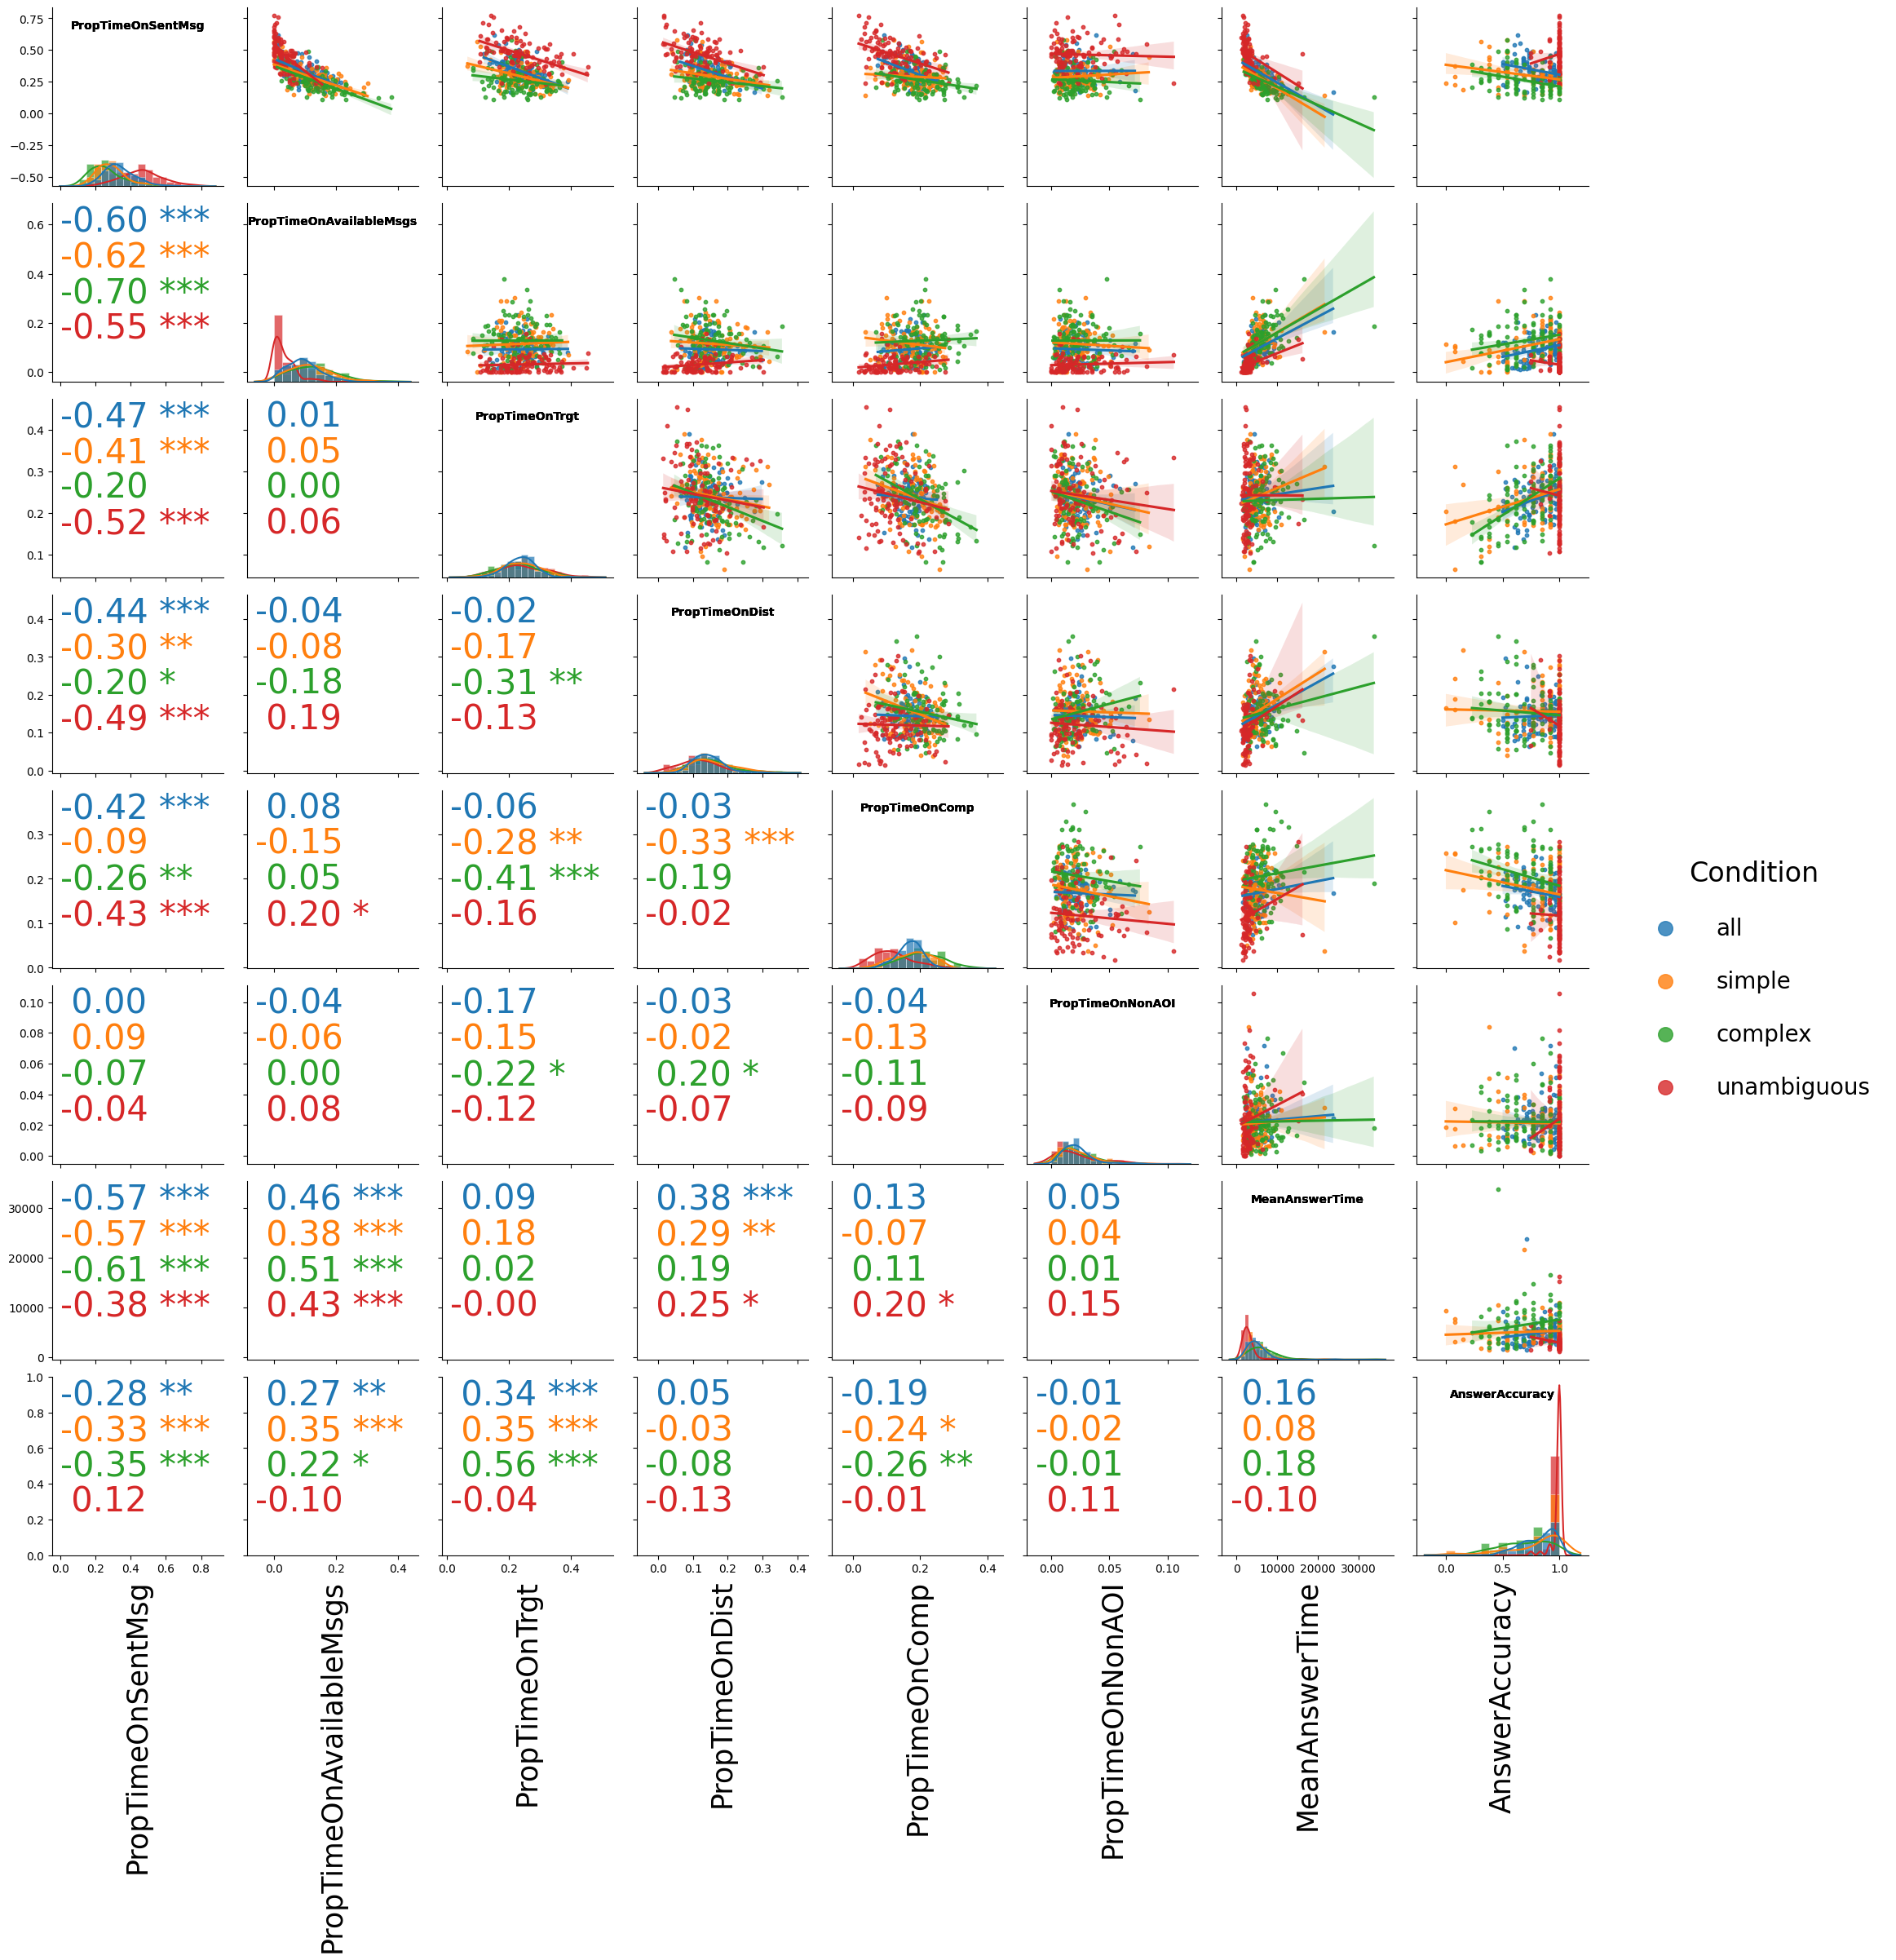
\includegraphics[width=0.95\textwidth]{images/pairwise_corr.png}
    \caption{Full pairwise correlation matrix for all conditions and features. The diagonal shows the distribution of the features. The top right triangle shows the scatter plots along with the regression lines. The bottom left triangle shows the correlation coefficients. Significance levels: * $p < 0.05$, ** $p < 0.01$, *** $p < 0.001$.}
    \label{fig:pairwise_corr_full}
\end{figure}